\section{Finite protected inner-polytopal supercodes}
\label{sec:finite-supercodes}

The previous sections reduce the universal problem to deletions.  We now show that every arbitrary source realization has a finite polytopal approximation on the correct side of the problem: it preserves every target word exactly and creates only smaller words beneath source words.

\begin{theorem}[Protected inner-polytopal supercode]
\label{thm:protected-supercode}
Let
\[
 \C=\code(U_1,\ldots,U_n;X)
\]
be a finite open convex code in a finite-dimensional affine space, and choose one atom witness $x_\rho$ for every $\rho\in\C$.  After deleting neurons that occur in no codeword, there exist a compact convex polytope $Q\Subset X$ and nonempty compact convex polytopes
\[
 P_i\Subset U_i\cap\operatorname{int}Q
\]
such that, for
\[
 \D=\code(\operatorname{int}P_1,\ldots,\operatorname{int}P_n;\operatorname{int}Q),
\]
one has
\[
 \boxed{\C\subseteq\D\subseteq\Delta(\C).}
\]
Every $x_\rho$ remains an exact witness for $\rho$, and $\C$ and $\D$ have the same maximal words.  Deleted trivial inactive neurons may be restored by choosing lower-dimensional polytopes with empty ambient interior.
\end{theorem}

\begin{proof}
First delete every neuron that belongs to no codeword.  This does not alter any nontrivial trunk, and such neurons may be restored at the end by polytopes with empty interior in the common ambient.  For each $\rho\in\C$, openness of
\[
 X\cap\bigcap_{i\in\rho}U_i
\]
provides a full-dimensional compact simplex $S_\rho$ with
\[
 x_\rho\in\operatorname{int}S_\rho,
 \qquad
 S_\rho\Subset X\cap\bigcap_{i\in\rho}U_i.
\]
The simplex is not required to lie in the atom $A_\rho$; excluded neurons may cover part of it.  Define
\[
 P_i=\conv\bigcup_{\rho\ni i}S_\rho.
\]
Every simplex in this union lies in the open convex set $U_i$, so $P_i\subset U_i$.  Compactness gives $P_i\Subset U_i$.  The union of the finitely many $P_i$ and protected witnesses is compact in the open convex set $X$.  Hence one may choose a compact polytope $Q\Subset X$ whose interior contains every $P_i$ and every witness.

If $i\in\rho$, then
\[
 x_\rho\in\operatorname{int}S_\rho\subseteq\operatorname{int}P_i.
\]
If $j\notin\rho$, then $x_\rho\notin U_j$, while $P_j\subset U_j$, so $x_\rho\notin P_j$.  Thus every target word survives exactly.

For arbitrary $x\in\operatorname{int}Q$, let
\[
 d(x)=\{i:x\in\operatorname{int}P_i\},
 \qquad
 c(x)=\{i:x\in U_i\}.
\]
Since $\operatorname{int}P_i\subset U_i$, one has $d(x)\subseteq c(x)$.  The source word $c(x)$ belongs to $\C$, so $d(x)\in\Delta(\C)$.  This proves $\D\subseteq\Delta(\C)$.  Every maximal word of $\C$ survives, while every word of $\D$ is contained in a source word; hence the maximal words agree.
\end{proof}

\begin{figure}[t]
\centering
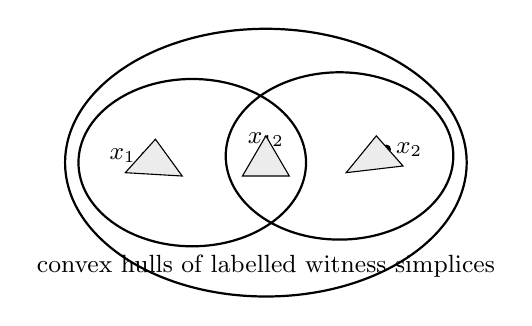
\begin{tikzpicture}[scale=.85,font=\small]
\draw[thick] (0,0) ellipse (3 and 2);
\draw[thick] (-1.1,0) ellipse (1.7 and 1.25);
\draw[thick] (1.1,.1) ellipse (1.7 and 1.25);
\fill (-1.8,.1) circle (2pt) node[left]{$x_1$};
\fill (1.8,.2) circle (2pt) node[right]{$x_2$};
\fill (0,.1) circle (2pt) node[above]{$x_{12}$};
\draw[fill=gray!15] (-2.1,-.15)--(-1.65,.35)--(-1.25,-.2)--cycle;
\draw[fill=gray!15] (1.2,-.15)--(1.65,.4)--(2.05,-.05)--cycle;
\draw[fill=gray!15] (-.35,-.2)--(0,.4)--(.35,-.2)--cycle;
\node at (0,-1.55) {convex hulls of labelled witness simplices};
\end{tikzpicture}
\caption{Protected supercode construction.  Each target word has a small source-contained simplex.  Neuron $i$ is the convex hull of all simplices whose labels contain $i$.  The selected atom witnesses remain exact.}
\label{fig:protected-supercode}
\end{figure}

\begin{remark}[Degenerate atoms]
A source atom may be lower dimensional or supported on several boundaries.  The construction requires only that its witness lies in the open intersection of the neurons that are active there.  The small simplex may cross excluded-neuron boundaries; inactive membership at the protected witness is nevertheless preserved because every new neuron polytope remains inside its source neuron.
\end{remark}

\begin{remark}[Finite but not exact]
The theorem replaces arbitrary curved fields by finitely many polytopes but generally produces a supercode.  The only errors are words obtained by deleting memberships from source words.  This one-sidedness is what makes the repair atlas in the next section possible.
\end{remark}
